\documentclass[12pt,letterpaper]{article}
\usepackage{graphicx,textcomp}
\usepackage{natbib}
\usepackage{setspace}
\usepackage{fullpage}
\usepackage{color}
\usepackage[reqno]{amsmath}
\usepackage{amsthm}
\usepackage{amssymb,enumerate}
\usepackage[all]{xy}
\usepackage{endnotes}
\usepackage{lscape}
\usepackage{float}
\newtheorem{com}{Comment}
\newtheorem{lem} {Lemma}
\newtheorem{prop}{Proposition}
\newtheorem{thm}{Theorem}
\newtheorem{defn}{Definition}
\newtheorem{cor}{Corollary}
\newtheorem{obs}{Observation}
\usepackage[compact]{titlesec}
\usepackage{dcolumn}
\usepackage{tikz}
\usetikzlibrary{arrows}
\usepackage{multirow}
\usepackage{xcolor}
\newcolumntype{.}{D{.}{.}{-1}}
\newcolumntype{d}[1]{D{.}{.}{#1}}
\definecolor{light-gray}{gray}{0.65}
\usepackage{url}
\usepackage{listings}
\usepackage{color}
 
\definecolor{codegreen}{rgb}{0,0.6,0}
\definecolor{codegray}{rgb}{0.5,0.5,0.5}
\definecolor{codepurple}{rgb}{0.58,0,0.82}
\definecolor{backcolour}{rgb}{0.95,0.95,0.92}
 
\lstdefinestyle{mystyle}{
    backgroundcolor=\color{backcolour},   
    commentstyle=\color{codegreen},
    keywordstyle=\color{magenta},
    numberstyle=\tiny\color{codegray},
    stringstyle=\color{codepurple},
    basicstyle=\footnotesize,
    breakatwhitespace=false,         
    breaklines=true,                 
    captionpos=b,                    
    keepspaces=true,                 
    numbers=left,                    
    numbersep=5pt,                  
    showspaces=false,                
    showstringspaces=false,
    showtabs=false,                  
    tabsize=2
}
 \lstset{style=mystyle}
\newcommand{\Sref}[1]{Section~\ref{#1}}
\newtheorem{hyp}{Hypothesis}

\title{Text as Data: Homework 1}
\date{August 15, 2017}
\author{Jeff Ziegler}

\begin{document}
\maketitle

\noindent \textit{In this homework assignment we're going to analyze the first presidential debate from the 2012 election.}  \\

\subsubsection*{Problem 1}
\textit{To analyze the debate, we first need to load the debate and parse the content.  On the coursewebsite, you'll find the file {\tt debate1.html}.  Download the file and open it in a browser. We will use {\tt BeautifulSoup} to parse HTML file containing the debate transcript.}

\begin{itemize}
\item \textit{Load the webpage into {\tt Python} and use {\tt BeautifulSoup} to create a searchable version of the debate. What tags can you use to identify statements?}

\lstinputlisting[language=Python, firstline=5, lastline=14]{WUSTL_HW1_JZ.py}

\item \textit{Note that not all of the statements contain information about the speaker. Devise a rule to assign the unlabeled statements to speakers. For substantive reasons, we would like to define a single statement as any \textit{uninterrupted} speech from a candidate. We'll say a candidate is interrupted when the transcript says that a new speaker has begun.  In other words, cross talk doesn't count as an interruption. Create a list with just the text (not the tags) of each statement as an element. Some statements are split among several tags; these will need to be concatenated according to the rule you devised above. Remember to filter out notes about audience behavior.}

\lstinputlisting[language=Python, firstline=16, lastline=64]{WUSTL_HW1_JZ.py}

\end{itemize}

\subsection*{Problem 2}
\textit{Now we're going to do some more preprocessing to create a dataset that includes useful information about our texts. We will use a curated dictionary list from Neal Caren. The positive words are at {\tt http://www.unc.edu/$\sim$ncaren/haphazard/positive.txt} and the negative words are at {\tt http://www.unc.edu/$\sim$ncaren/haphazard/negative.txt}.}
\begin{itemize}
\item Load the positive and negative words into {\tt python}. Use the {\tt porter}, {\tt snowball} and {\tt lancaster} stemmers from the {\tt nltk} package to create stemmed versions of the dictionaries.

\lstinputlisting[language=Python, firstline=70, lastline=113]{WUSTL_HW1_JZ.py}

\item \textit{Using the original and stemmed dictionaries, we're going to create a statement by statement data set of the speech.
The data set should have the following columns:}
\begin{itemize}
\item[1)] \textit{Statement number (place in debate)}
\item[2)] \textit{Speaker}
\item[3)] \textit{Number of non-stop words spoken}
\item[4)] \textit{Number of positive words}
\item[5)] \textit{Number of negative words}
\item[6)] \textit{Number of lancaster stemmed positive words}
\item[7)] \textit{Number of lancaster stemmed negative words}
\item[8)] \textit{Number of porter stemmed positive words}
\item[9)] \textit{Number of porter stemmed negative words}
\item[10)] \textit{Number of snowball stemmed positive words}
\item[11)] \textit{Number of snowball stemmed negative words}
\end{itemize}
\end{itemize}

\noindent \textit{To create the data set, create a set of nested dictionaries that map each statement in the list created in Problem 1 to the each of the attributes described above. To  calculate the values for items 3 - 11 above, you'll need to do the following to each statement:}
\begin{itemize}
\item[-]  \textit{Discard punctuation}
\item[-]  \textit{Remove capitalization}
\item[-]  \textit{Remove stop words with the list of words provided here: \\
{\tt `http://jmlr.org/papers/volume5/lewis04a/a11-smart-stop-list/english.stop'}}
\item[-]  \textit{Tokenize the words}
\item[-] \textit{Apply each of the stemmers, determining which of the words appear in the corresponding stemmed dictionaries}
\end{itemize}

\noindent \textit{Write your dataset as a .csv file and save it to a working directory. Turn it in with your homework.}

\lstinputlisting[language=Python, firstline=114]{WUSTL_HW1_JZ.py}

\subsection*{Problem 3}

Using our new data set, let's make some observations about the debate
\begin{itemize}
\item[-] Load the data into {\tt R}
\end{itemize}

\lstinputlisting[language=R, firstline=1, lastline=4]{WUSTL_HW1_JZ.r}

\begin{itemize}
\item[-] Create a visualization that compares the overall positive and negative word rate for Obama, Romney, and Lehrer.  What patterns do you notice?  There is no one right answer, be creative!
\end{itemize}

\lstinputlisting[language=R, firstline=5, lastline=19]{WUSTL_HW1_JZ.r}

\begin{figure}[H]
  \caption{\footnotesize{Unstemmed word rate.}}
  \centering
   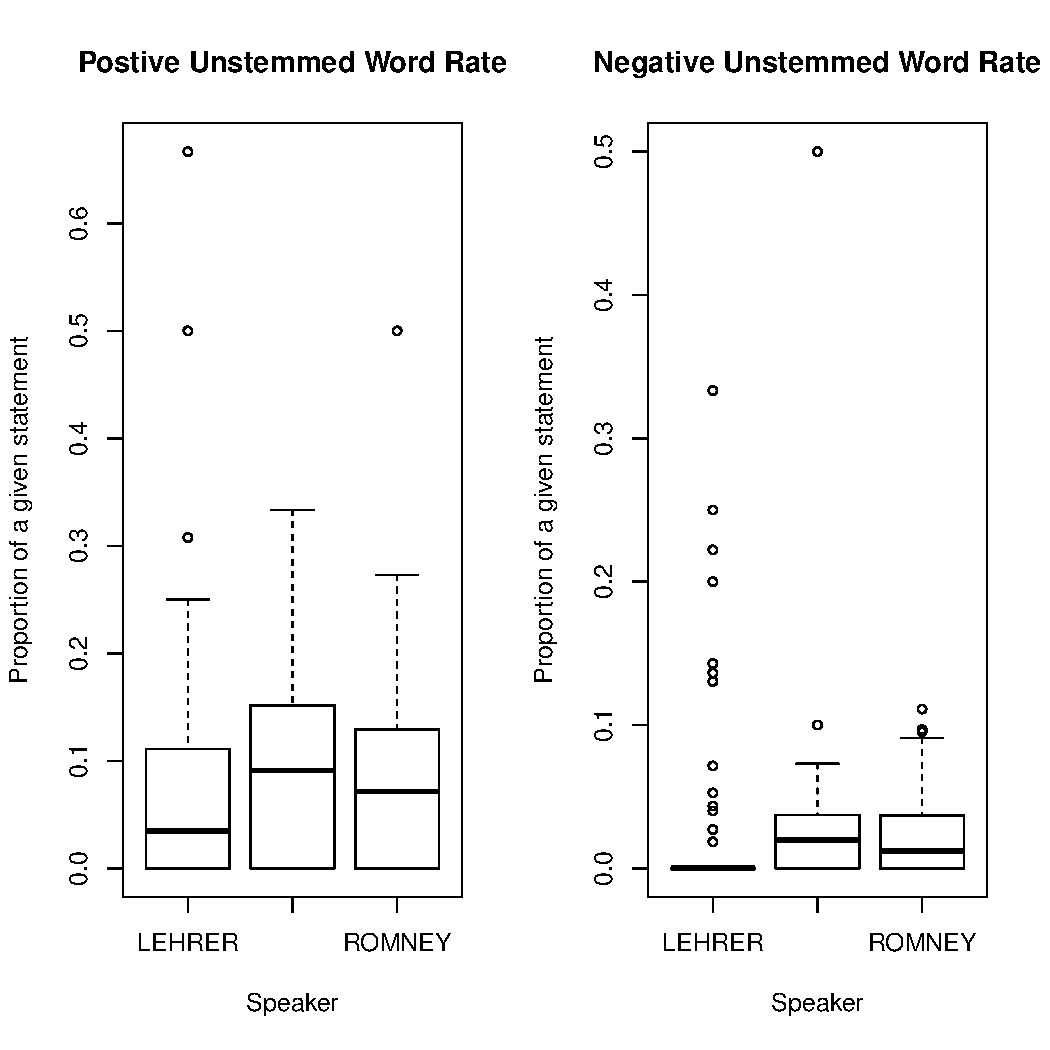
\includegraphics[width=.65\linewidth]{HW1wordRatePlot.pdf}\\
    \footnotesize{Figure notes: Obama is center speaker category that is missing.}
\end{figure}

\begin{itemize}
\item[-] Using your data set, examine trends in each candidate's statements and Lehrer's speeches.  Do you notice any
\begin{itemize}
\item[i)] Trends in the measured tone?
\end{itemize}
\end{itemize}

\lstinputlisting[language=R, firstline=21, lastline=34]{WUSTL_HW1_JZ.r}

\begin{table}[H]
\centering
  \caption{\footnotesize{Regression results, positive tone by speaker overtime.}}
\begin{tabular}{rrrrr}
  \hline
 & Estimate & Std. Error & t value & Pr($>$$|$t$|$) \\ 
  \hline
(Intercept) & 0.0561 & 0.0302 & 1.86 & 0.0667 \\ 
  Statement Number & 0.0005 & 0.0003 & 1.62 & 0.1090 \\ 
  Speaker: Romney & 0.0367 & 0.0407 & 0.90 & 0.3689 \\ 
  Statement Number:Romney& -0.0005 & 0.0004 & -1.27 & 0.2058 \\ 
   \hline
\end{tabular}
\end{table}

\begin{itemize}
\item[ii)] Response to the other candidate's tone (examining who spoke previously)?
\end{itemize}

\lstinputlisting[language=R, firstline=36, lastline=48]{WUSTL_HW1_JZ.r}

\begin{table}[H]
\centering
  \caption{\footnotesize{Regression results, positive tone by previous speaker overtime.}}
\begin{tabular}{rrrrr}
  \hline
 & Estimate & Std. Error & t value & Pr($>$$|$t$|$) \\ 
  \hline
(Intercept) & 0.1142 & 0.0458 & 2.49 & 0.0144 \\ 
Statement Number & 0.0001 & 0.0005 & 0.21 & 0.8325 \\ 
Previous speaker & -0.0255 & 0.0314 & -0.81 & 0.4191 \\ 
  Statement Number:Previous speaker  & 0.0000 & 0.0004 & 0.12 & 0.9076 \\ 
   \hline
\end{tabular}\\
    \footnotesize{Notes: Assume moderator influences tone of candidates, but don't care if moderator is influenced by respondents.}
\end{table}

\begin{itemize}
\item[iii)] Overall interesting patterns? (this is an intentionally vague question)
\end{itemize}

\lstinputlisting[language=R, firstline=49]{WUSTL_HW1_JZ.r}

\begin{table}[H]
\centering
  \caption{\footnotesize{Regression results, positive tone by previous speaker (only candidates) overtime.}}
\begin{tabular}{rrrrr}
  \hline
 & Estimate & Std. Error & t value & Pr($>$$|$t$|$) \\ 
  \hline
(Intercept) & 0.2261 & 0.1692 & 1.34 & 0.1848 \\ 
  Statement Number & -0.0019 & 0.0018 & -1.07 & 0.2857 \\ 
  Previous speaker & -0.0374 & 0.0651 & -0.58 & 0.5667 \\ 
  Statement Number:Previous speaker & 0.0006 & 0.0007 & 0.86 & 0.3938 \\ 
   \hline
\end{tabular}\\
    \footnotesize{Notes: Remove moderator speech, and assume that moderator doesn't influence tone of respondents.}
\end{table}





\end{document}
